% Options for packages loaded elsewhere
\PassOptionsToPackage{unicode}{hyperref}
\PassOptionsToPackage{hyphens}{url}
%
\documentclass[
  12pt,
  a4paper,
]{scrreprt}
\usepackage{amsmath,amssymb}
\usepackage{lmodern}
\usepackage{setspace}
\usepackage{iftex}
\ifPDFTeX
  \usepackage[T1]{fontenc}
  \usepackage[utf8]{inputenc}
  \usepackage{textcomp} % provide euro and other symbols
\else % if luatex or xetex
  \usepackage{unicode-math}
  \defaultfontfeatures{Scale=MatchLowercase}
  \defaultfontfeatures[\rmfamily]{Ligatures=TeX,Scale=1}
  \setmainfont[Ligatures=TeX]{PT Serif}
  \setsansfont[Ligatures=TeX,Scale=MatchLowercase]{PT Sans}
  \setmonofont[Scale=MatchLowercase,Scale=0.9]{PT Mono}
\fi
% Use upquote if available, for straight quotes in verbatim environments
\IfFileExists{upquote.sty}{\usepackage{upquote}}{}
\IfFileExists{microtype.sty}{% use microtype if available
  \usepackage[]{microtype}
  \UseMicrotypeSet[protrusion]{basicmath} % disable protrusion for tt fonts
}{}
\usepackage{xcolor}
\setlength{\emergencystretch}{3em} % prevent overfull lines
\providecommand{\tightlist}{%
  \setlength{\itemsep}{0pt}\setlength{\parskip}{0pt}}
\setcounter{secnumdepth}{5}
\ifLuaTeX
\usepackage[english]{babel}
\else
\usepackage[bidi=default]{babel}
\fi
\babelprovide[main,import]{russian}
\babelprovide[import]{english}
% get rid of language-specific shorthands (see #6817):
\let\LanguageShortHands\languageshorthands
\def\languageshorthands#1{}
\usepackage{indentfirst}
\usepackage{float}
\floatplacement{figure}{H}
\ifLuaTeX
  \usepackage{selnolig}  % disable illegal ligatures
\fi
\usepackage[style=gost-numeric,parentracker=true,backend=biber,hyperref=auto,language=auto,autolang=other*,citestyle=gost-numeric]{biblatex}
\addbibresource{bib/cite.bib}
\IfFileExists{bookmark.sty}{\usepackage{bookmark}}{\usepackage{hyperref}}
\IfFileExists{xurl.sty}{\usepackage{xurl}}{} % add URL line breaks if available
\urlstyle{same} % disable monospaced font for URLs
\hypersetup{
  pdftitle={Отчёт по лабораторной работе №8},
  pdfauthor={Рыжкова Ульяна Валерьевна},
  pdflang={ru-RU},
  hidelinks,
  pdfcreator={LaTeX via pandoc}}

\title{Отчёт по лабораторной работе №8}
\usepackage{etoolbox}
\makeatletter
\providecommand{\subtitle}[1]{% add subtitle to \maketitle
  \apptocmd{\@title}{\par {\large #1 \par}}{}{}
}
\makeatother
\subtitle{Операционные системы}
\author{Рыжкова Ульяна Валерьевна}
\date{}

\begin{document}
\maketitle

\renewcommand*\contentsname{Содержание}
{
\setcounter{tocdepth}{2}
\tableofcontents
}
\listoffigures
\listoftables
\setstretch{1.5}

\hypertarget{ux446ux435ux43bux44c-ux440ux430ux431ux43eux442ux44b}{%
\chapter{Цель
работы}\label{ux446ux435ux43bux44c-ux440ux430ux431ux43eux442ux44b}}

Ознакомиться с текстовым редактором vi и получить практические навыки
работы с ним

\hypertarget{ux437ux430ux434ux430ux43dux438ux435-1.-ux441ux43eux437ux434ux430ux43dux438ux435-ux43dux43eux432ux43eux433ux43e-ux444ux430ux439ux43bux430-ux441-ux438ux441ux43fux43eux43bux44cux437ux43eux432ux430ux43dux438ux435ux43c-vi}{%
\chapter{Задание 1. Создание нового файла с использованием
vi}\label{ux437ux430ux434ux430ux43dux438ux435-1.-ux441ux43eux437ux434ux430ux43dux438ux435-ux43dux43eux432ux43eux433ux43e-ux444ux430ux439ux43bux430-ux441-ux438ux441ux43fux43eux43bux44cux437ux43eux432ux430ux43dux438ux435ux43c-vi}}

\begin{enumerate}
\def\labelenumi{\arabic{enumi}.}
\tightlist
\item
  Создаём каталог и переходим в него
\end{enumerate}

\begin{figure}
\hypertarget{fig:001}{%
\centering
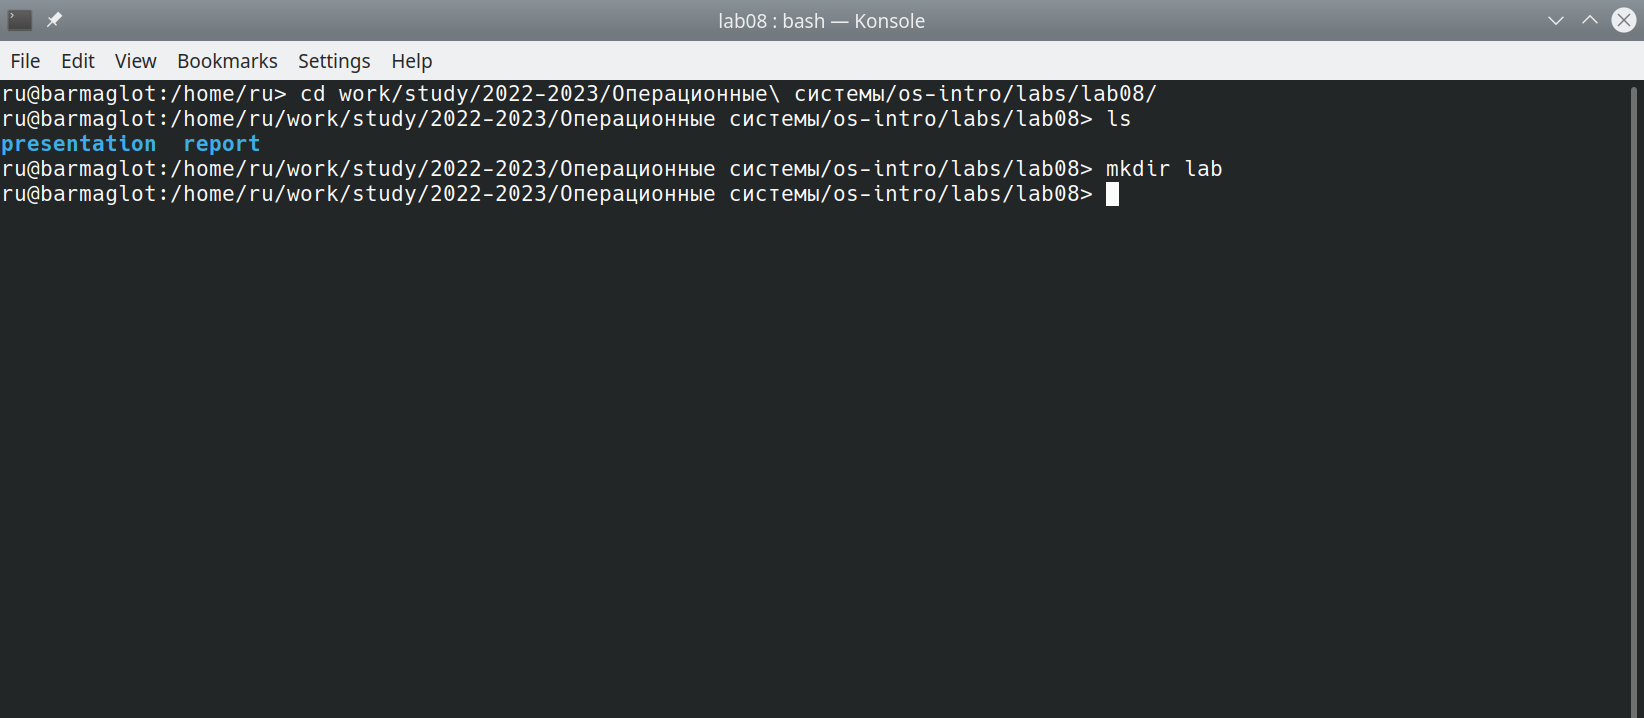
\includegraphics[width=1\textwidth,height=\textheight]{image/1.png}
\caption{Создание каталога}\label{fig:001}
}
\end{figure}

\begin{enumerate}
\def\labelenumi{\arabic{enumi}.}
\setcounter{enumi}{1}
\tightlist
\item
  Создаём файл с помощью команды vi hello.sh
\end{enumerate}

\begin{figure}
\hypertarget{fig:002}{%
\centering
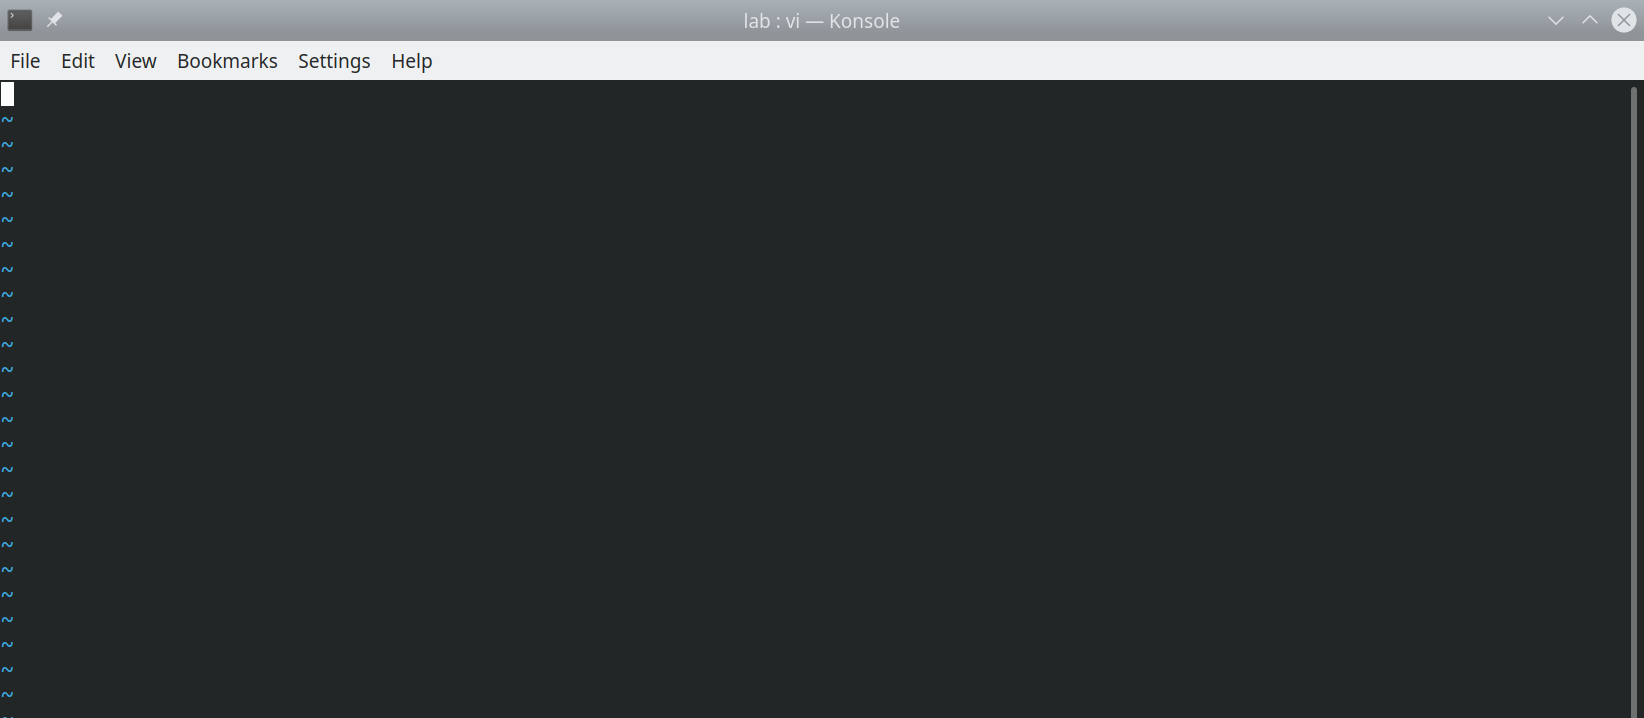
\includegraphics[width=1\textwidth,height=\textheight]{image/2.png}
\caption{Новый файл}\label{fig:002}
}
\end{figure}

\begin{enumerate}
\def\labelenumi{\arabic{enumi}.}
\setcounter{enumi}{2}
\tightlist
\item
  Вводим текст, и с помощью комбинации :wq сохраняем изменения и выходим
  из редактора
\end{enumerate}

\begin{figure}
\hypertarget{fig:003}{%
\centering
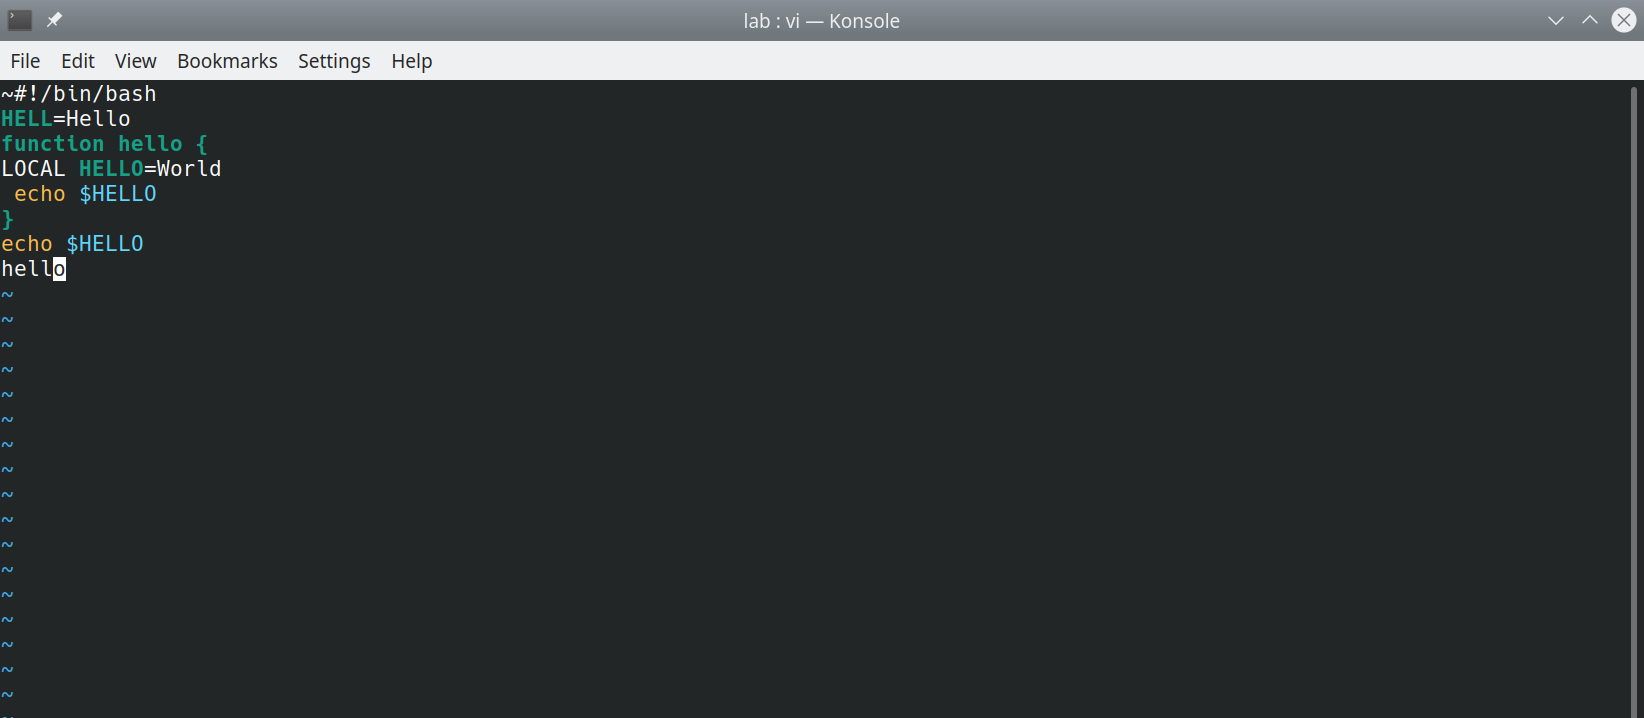
\includegraphics[width=1\textwidth,height=\textheight]{image/4.png}
\caption{Сохранённый текст}\label{fig:003}
}
\end{figure}

\begin{enumerate}
\def\labelenumi{\arabic{enumi}.}
\setcounter{enumi}{3}
\tightlist
\item
  Делаем файл исполняемым
\end{enumerate}

\begin{figure}
\hypertarget{fig:004}{%
\centering
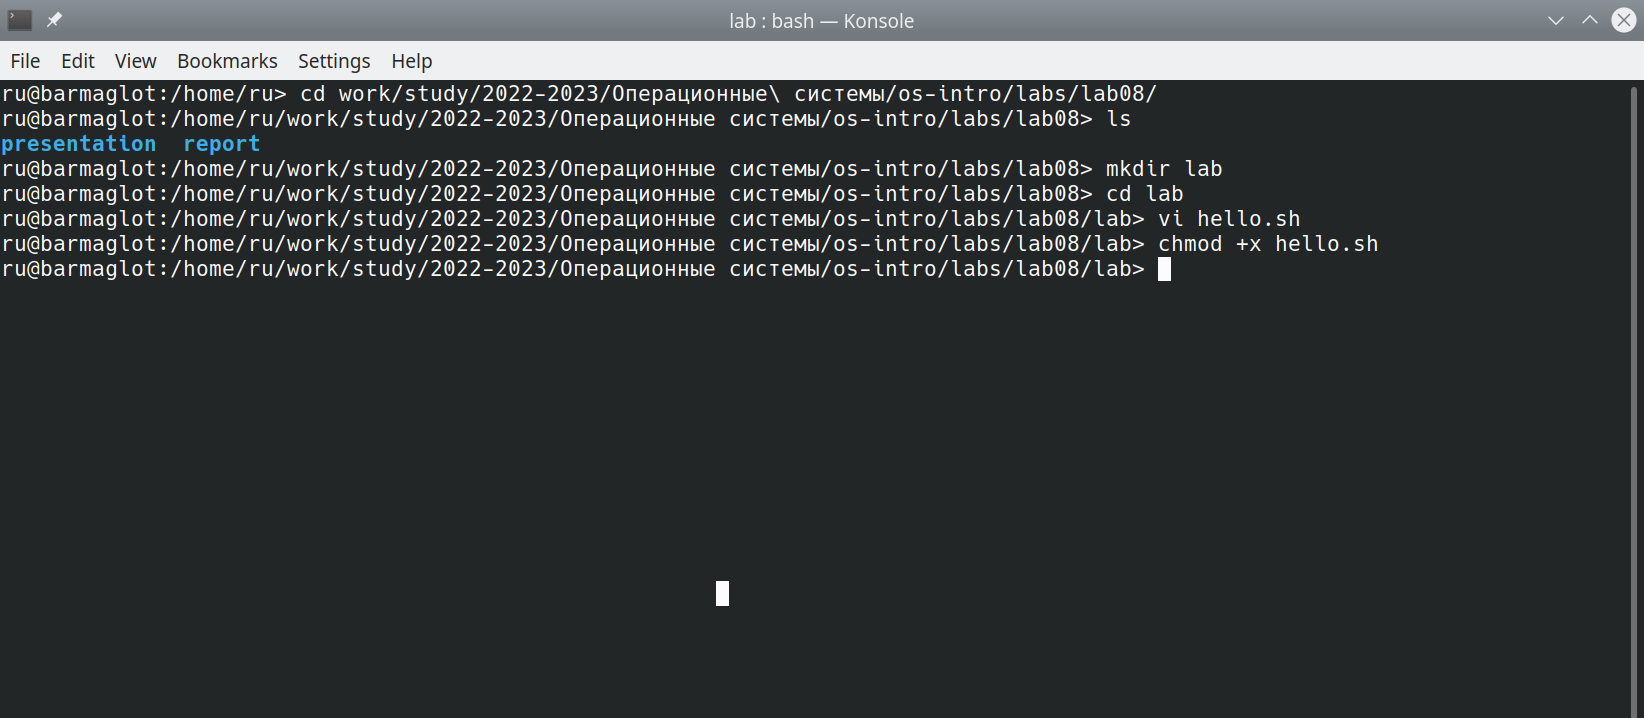
\includegraphics[width=1\textwidth,height=\textheight]{image/3.png}
\caption{Команда chmod +x}\label{fig:004}
}
\end{figure}

\hypertarget{ux437ux430ux434ux430ux43dux438ux435-2.-ux440ux435ux434ux430ux43aux442ux438ux440ux43eux432ux430ux43dux438ux435-ux441ux443ux449ux435ux441ux442ux432ux443ux44eux449ux435ux433ux43e-ux444ux430ux439ux43bux430}{%
\chapter{Задание 2. Редактирование существующего
файла}\label{ux437ux430ux434ux430ux43dux438ux435-2.-ux440ux435ux434ux430ux43aux442ux438ux440ux43eux432ux430ux43dux438ux435-ux441ux443ux449ux435ux441ux442ux432ux443ux44eux449ux435ux433ux43e-ux444ux430ux439ux43bux430}}

\begin{enumerate}
\def\labelenumi{\arabic{enumi}.}
\item
  Вызвав vi на редактирование файла, устанавливаем курсор в конец слова
  HELL 2-ой строки, используя комбинацию 2G и 5 пробелов
\item
  Переходим в режим вставки, нажав i, добавляем букву O, и, нажав esc,
  возвращаемся в командный режим
\end{enumerate}

\begin{figure}
\hypertarget{fig:005}{%
\centering
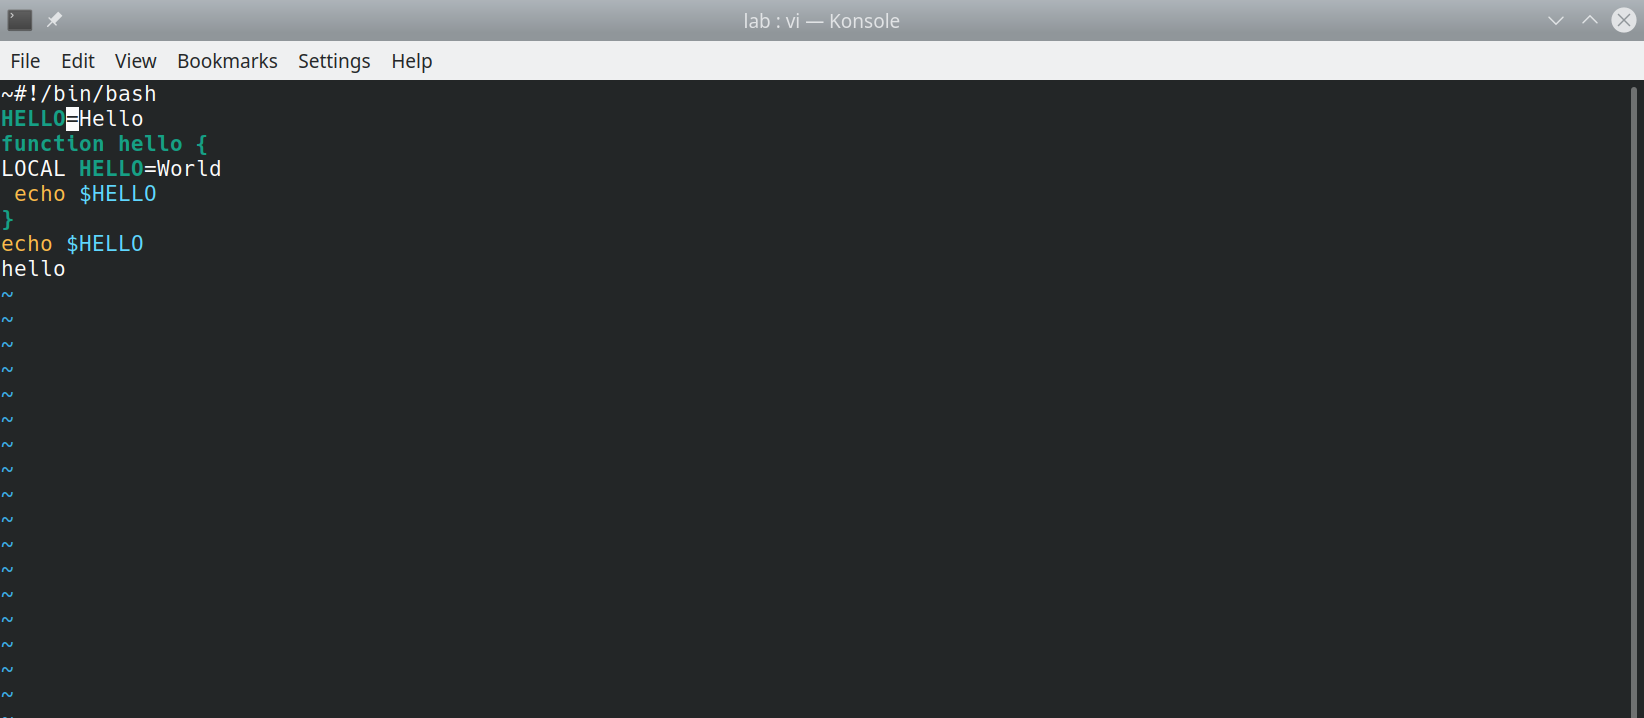
\includegraphics[width=1\textwidth,height=\textheight]{image/5.png}
\caption{Ввели слово HELLO}\label{fig:005}
}
\end{figure}

\begin{enumerate}
\def\labelenumi{\arabic{enumi}.}
\setcounter{enumi}{2}
\tightlist
\item
  Переходим в 4-ую строку (комбинация 4G) и стираем слово LOCAL
  (комбинация dw)
\end{enumerate}

\begin{figure}
\hypertarget{fig:006}{%
\centering
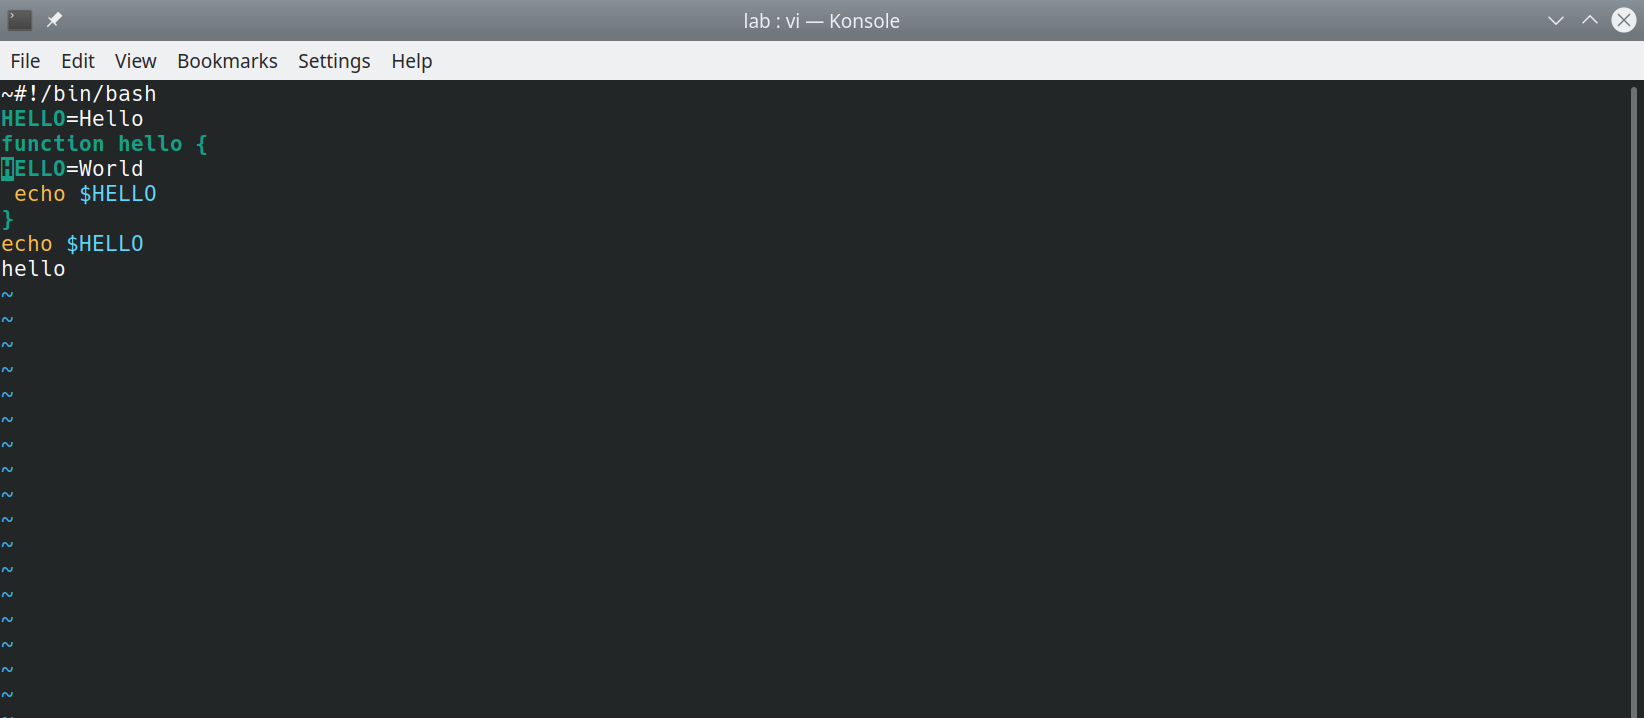
\includegraphics[width=1\textwidth,height=\textheight]{image/6.png}
\caption{Удалили слово LOCAL}\label{fig:006}
}
\end{figure}

\begin{enumerate}
\def\labelenumi{\arabic{enumi}.}
\setcounter{enumi}{3}
\tightlist
\item
  Переходим в режим вставки (i), вводим слово `local', и возвращаемся в
  командный режим (esc)
\end{enumerate}

\begin{figure}
\hypertarget{fig:007}{%
\centering
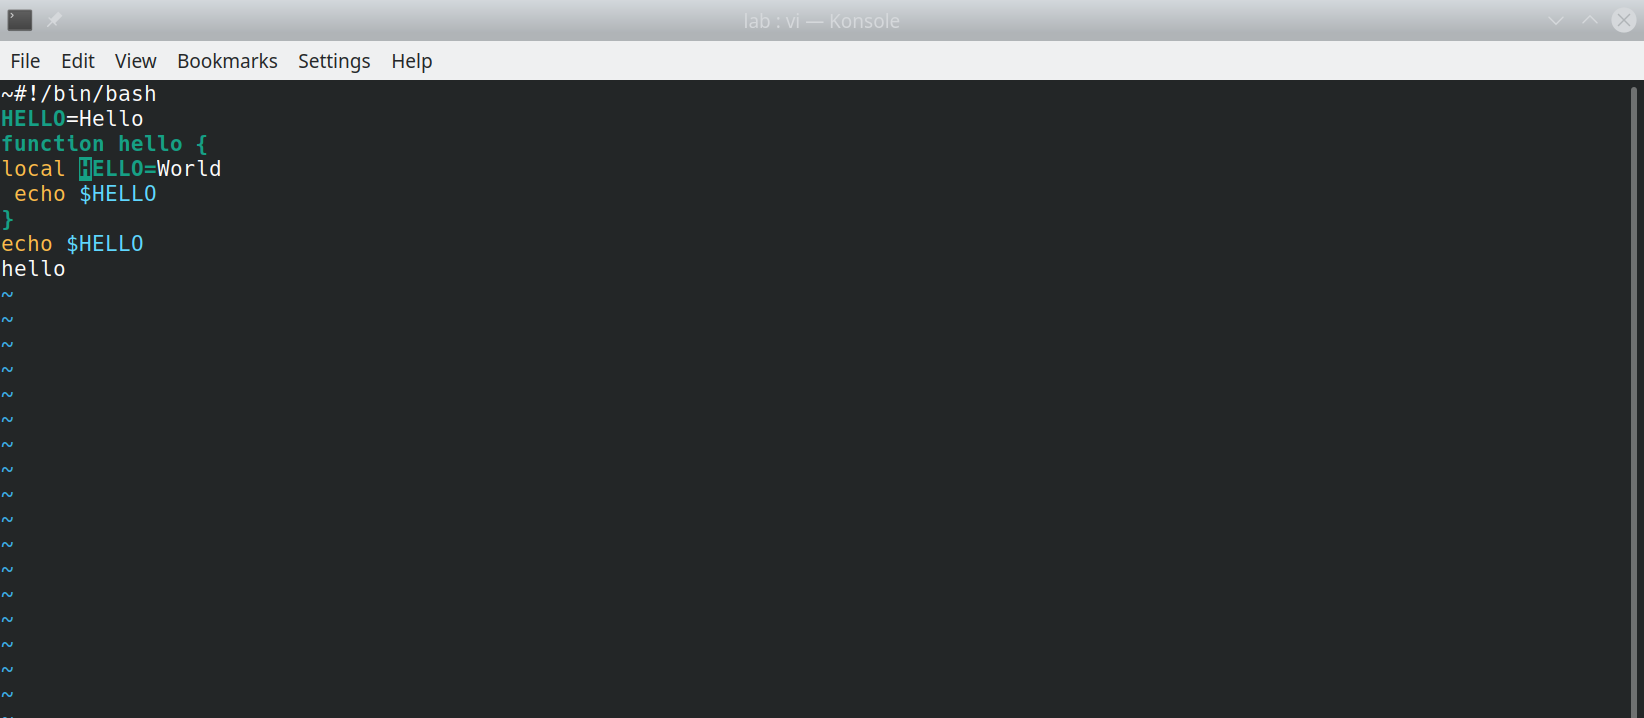
\includegraphics[width=1\textwidth,height=\textheight]{image/7.png}
\caption{Ввели слово local}\label{fig:007}
}
\end{figure}

\begin{enumerate}
\def\labelenumi{\arabic{enumi}.}
\setcounter{enumi}{4}
\item
  Перемещаемся в последнюю строку (G), вставляем пустую строку (о) и
  вводим текст
\item
  Удаляем последнюю строку с помощью комбинации dd. Отменяем последнее
  действие клавишей u
\item
  Вводим :wq, чтобы сохранить изменения и выйти из файла.
\end{enumerate}

\hypertarget{ux43aux43eux43dux442ux440ux43eux43bux44cux43dux44bux435-ux432ux43eux43fux440ux43eux441ux44b}{%
\chapter{Контрольные
вопросы}\label{ux43aux43eux43dux442ux440ux43eux43bux44cux43dux44bux435-ux432ux43eux43fux440ux43eux441ux44b}}

\begin{enumerate}
\def\labelenumi{\arabic{enumi}.}
\item
  Редактор vi имеет три режима работы:

  \begin{itemize}
  \tightlist
  \item
    Командный режим - ввод команд и навигация
  \item
    Режим вставки - редактирование содержимого файла
  \item
    Режим последней строки - запись изменений и выход из редактора
  \end{itemize}
\item
  Комбинация :q! выйти из редактора без записи изменений.
\item
  Команды позиционирования:

  \begin{itemize}
  \tightlist
  \item
    0 (ноль) - переход в начало строки
  \item
    \$ - переход в конец строки
  \item
    G - переход в конец файла
  \item
    nG - переход на строку с номером n
  \end{itemize}
\item
  Под разделителями понимаются пробел и табуляция при использовании W и
  B. При w и b - также любые знаки пунктуации.
\item
  Переход в начало файла выполняется с использованием комбинации 1G, в
  конец файла: G.
\item
  Вставка текста:

  \begin{itemize}
  \tightlist
  \item
    а - вставка после курсора
  \item
    А - вставка в конец строки
  \item
    i - вставка перед курсором
  \item
    ni - вставка n раз
  \item
    l - вставка в начало строки
  \end{itemize}
\end{enumerate}

Вставка строки: * о - вставка под курсором * О - вставка над курсором

Удаление текста: * х - удаление 1 символа в буфер * dw - удаление 1
слова в буфер * d\$ - удаление в буфер текста от курсора до конца строки
* d0 - удаление в буфер текста от начала строки до позиции курсора * dd
- удаление в буфер одной строки * ndd - удаление в буфер n строк

Отмена и повтор произведённых действий: * u - отмена последнего действия
* . - повтор последнего действия

Копирование текста в буфер: * Y - копирование строки в буфер * nY -
копирование n строк в буфер * yw - копирование слова в буфер

Вставка текста из буфера: * р - вставка из буфера после курсора * Р -
вставка из буфера перед курсором

Замена текста: * cw - замена слова * ncw - замена n слов * с\$ - замена
текста от курсора до конца строки * r - замена слова * R - замена текста

Поиск текста: * /текст - поиск вперёд по тексту указанной строки
символов текст * ?текст - поиск назад по тексту указанной строки
символов текст

\begin{enumerate}
\def\labelenumi{\arabic{enumi}.}
\setcounter{enumi}{6}
\item
  i -\textgreater{} ввод необходимого количества символов \$.
\item
  Отмена последнего действия осуществляется с помощью клавиши u.
\item
  Команды редактирования в режиме командной строки делятся на 2 группы:
  копирование и перемещение текста; запись в файл и выход из редактора.
\item
  Клавиша \$ осуществляет переход в конец строки
\item
  Опции vi позволяют настроить рабочую среду. Для их задания
  используется команда set в режиме последней строки:

  \begin{itemize}
  \tightlist
  \item
    :set all - вывод полного списка опций
  \item
    :set nu - вывод номера строк
  \item
    :set list - вывод невидимых символов
  \item
    :set ic - не учитывать регистр при поиске
  \end{itemize}
\end{enumerate}

Для отказа от использования опции, в команде set перед именем опции надо
поставить no.

\begin{enumerate}
\def\labelenumi{\arabic{enumi}.}
\setcounter{enumi}{11}
\item
  Если в левом нижнем углу написано INSERT, то мы в режиме вставки. Если
  курсор находится в конце файла и мы видим двоеточие, то это режим
  командной строки. В остальных случаях - командный режим.
\item
  Взаимосвязь режимов работы:
\end{enumerate}

Командный режим * Режим вставки * Режим последней строки

\hypertarget{ux432ux44bux432ux43eux434ux44b}{%
\chapter{Выводы}\label{ux432ux44bux432ux43eux434ux44b}}

Я освоила базовый функционал текстового редактора vi
